\documentclass{standalone}

\usepackage{tikz}

\usepackage{verbatim}
\usetikzlibrary{arrows,shapes,shadows,calc}

\definecolor{blue@O4S}{RGB}{0, 41, 69}
\definecolor{emph@O4S}{RGB}{0, 93, 137}
\definecolor{red@O4S}{RGB}{127,0,0}
\definecolor{gray@O4S}{RGB}{112, 112, 112}


\begin{document}

  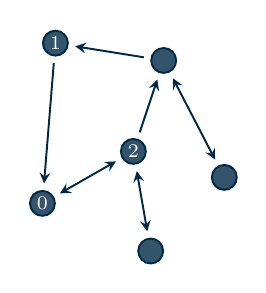
\begin{tikzpicture}[scale=1, font=\scriptsize]
  \tikzstyle{vertex}=[draw=blue@O4S,line width=0.7pt, circle, fill=blue@O4S!80, 
                                minimum size=9pt,inner sep=0pt]
  \tikzstyle{und_edge} = [draw,<->, stealth-stealth, blue@O4S, shorten >=2.4pt,shorten <=2.4pt,line width=0.7pt]
  \tikzstyle{dir_edge} = [draw,->, -stealth, blue@O4S, shorten >=2.4pt,shorten <=2.4pt,line width=0.7pt]


  % constants
  \def \NodeDistX {5.5}
  \def \NodeDistY {5.5}


    \coordinate(A) at (0.40*\NodeDistX, 0.35*\NodeDistY);
    \coordinate(B) at (0.65*\NodeDistX, 0.24*\NodeDistY);
    \coordinate(C) at (0.61*\NodeDistX, 0.47*\NodeDistY);
    \coordinate(D) at (0.68*\NodeDistX, 0.68*\NodeDistY);
    \coordinate(E) at (0.43*\NodeDistX, 0.72*\NodeDistY);
    \coordinate(F) at (0.82*\NodeDistX, 0.41*\NodeDistY);
    
    
    % Draw the vertices
    \foreach \pos/\name in 
        {
          {(A)/a},
          {(B)/b},
          {(C)/c},
          {(D)/d},
          {(E)/e},
          {(F)/f}%
        }
        \node[vertex] (\name) at \pos {}; % name and pos are assigned via foreach loop

      \node[text = white] at (A) {$0$};
      \node[text = white] at (C) {$2$};
      \node[text = white] at (E) {$1$}; % name and pos are assigned via foreach loop
%      \node[text = black, shift={(-0.05,-0.35)}] at (A) {$c_i, A_i, X_i$}; % name and pos are assigned via foreach loop

    % Connect vertices with edges
    \foreach \source/ \dest in 
      {
        a/c,
%        a/e,
        b/c,
%        c/d,
%        d/e,
        d/f%
      }
      \path[und_edge] (\source) -- (\dest);
    
    \foreach \source/ \dest in 
      {
%        a/c,
        e/a,
%        b/c,
        c/d,
        d/e%,
%        d/f%
      }
      \path[dir_edge] (\source) -- (\dest);

\end{tikzpicture}

\end{document}
